\begin{center}
    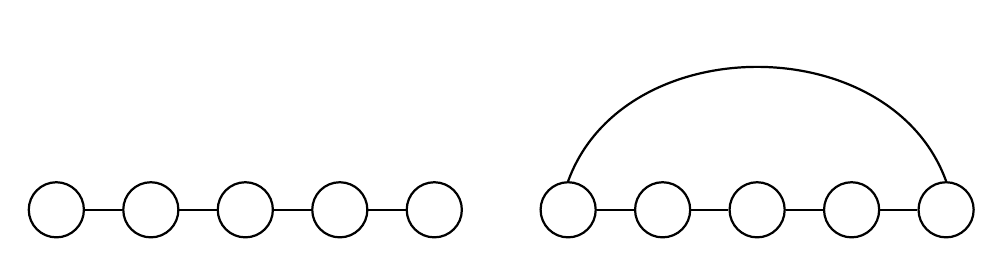
\begin{tikzpicture}[
        vertice/.style={
            circle,
            draw,
            minimum size=7mm,
            inner sep=0pt,
            line width=0.8pt
        },
        arista/.style={line width=0.8pt}
    ]
    
        % Grafo izquierdo: camino P5
        \foreach \i in {0,...,4} {
            \node[vertice] (p\i) at ({1.2*\i},0) {};
        }
    
        % Grafo derecho: ciclo C5
        \foreach \i in {0,...,4} {
            \node[vertice] (c\i) at ({6.5+1.2*\i},0) {};
        }
    
        % Aristas horizontales
        \foreach \a/\b in {0/1,1/2,2/3,3/4} {
            \draw[arista] (p\a) -- (p\b);
            \draw[arista] (c\a) -- (c\b);
        }
    
        % Arista curva del segundo grafo
        \draw[arista]
            (c0.north) to[out=70,in=110,looseness=1.1]
            (c4.north);
    
    \end{tikzpicture}
\end{center}